\chapter{Cascade of regulation - The Langevin equation}

\section{Intrinsic noise in a single gene using the Langevin approach}

In the Langevin approach, a term representing the noise of the system is added to the deterministic equations instead of considering the transition rates between states explicitely. Knowing some of the statistical properties of the noise term will allow us to find the noise in the number of species. In this section we will use the Langevin approach to find the intrinsic noise for a single gene.

Consider the model used on section \ref{sec:mas-single_gene}. For each of the deterministic equations (eqs. \label{eq:mas-simple_det_1} and \label{eq:mas-simple_det_2}), a stochastic process is added that accounts for the intrinsic noise. Including the terms $\mu_1(t)$ and $\mu_2(t)$ results in

\begin{align}
  \dot{n_1}(t) &= k_rd-\gamma_rn_1(t) + \mu_1(t)\label{eq:lan-simple_1},\\
  \dot{n_2}(t) &= k_pn_1(t)-\gamma_pn_2(t) + \mu_2(t)\label{eq:lan-simple_2}.
\end{align}

Now $n_1(t)$ and $n_2(t)$ are stochastic processes. We need to have some information of the noise terms in order to proceed. First, as we saw in chapter \ref{ch:master}, the averages must follow the deterministic behavior. By taking averages on both sides of eqs. \label{eq:lan-simple_1} - \label{eq:lan-simple_2} and imposing this condition we get

\begin{equation*}
  \langle\mu_r\rangle(t) = \langle\mu_r\rangle(t) = 0.
\end{equation*}

Also, assuming white noise statistics, the autocorrelations are given by

\begin{align}
  \langle\mu_1(t)\mu_1(t+\tau)\rangle &= q_1\delta(\tau),\label{eq:lan-simple_cor1} \\
  \langle\mu_2(t)\mu_2(t+\tau)\rangle &= q_2\delta(\tau). \label{eq:lan-simple_cor2}
\end{align}

This means that we will assume that there is no correlation between the values of the noise term at different times. The coefficients $q_1$ and $q_2$ determine the strenght of the noise and will be treated later. Also, the intrinsic noise must be fully uncorrelated among mRNA and proteins, hence

\begin{equation}
  \langle\mu_1(t)\mu_2(t+\tau)\rangle = 0. \label{eq:lan-simple_cor12}
\end{equation}

We will use eqs. \eqref{eq:lan-simple_cor1} - \eqref{eq:lan-simple_cor12} to find the noise in mRNA and protein numbers. Define the difference with respect to steady state average as $\delta n_1$ and $\delta n_2$, i.e. $\delta n_i \coloneqq n_i - \langle n_i\rangle_s$, for $i=1,2$. In terms of these quantities the eqs. become

\begin{align}
  \dot{\delta n_1}(t) &= -\gamma_r\delta n_1(t) + \mu_1(t)\label{eq:lan-simple_d1},\\
  \dot{\delta n_2}(t) &= k_p\delta n_1(t) -\gamma_p\delta n_2(t) + \mu_2(t)\label{eq:lan-simple_d2}.
\end{align}

Fourier transforming and using the fact that $\left[\mathscr{F}(\dot{x}(t))\right](\omega) = i\omega \hat{x}$, where $\hat{x}\coloneqq\mathscr{F}(x)$ we get 

\begin{equation}
  \delta\hat{n}_1(\omega) = \frac{\hat{\mu}_1(\omega)}{\gamma_r+i\omega},\quad\quad \delta\hat{n}_2(\omega) = \frac{\delta\hat{n}_1(\omega) + \hat{\mu}_2(\omega)}{\gamma_p+i\omega}.
\end{equation}

Taking the average of the square norm of the first expression we obtain the power spectrum for $\delta n_1$

\begin{equation*}
  \langle|\delta\hat{n}_1|^2\rangle = \frac{\langle|\hat{\mu}_1|^2\rangle}{\omega^2+\gamma^2} = \frac{q_1}{\omega^2+\gamma_r^2},
\end{equation*}

because by using the Wiener-Khinchin theorem (eq. \eqref{eq:con-wkth}) and eq. \eqref{eq:lan-simple_cor1} we obtain $\langle|\hat{\mu}_1|^2\rangle = q_1^2$. Making the inverse Fourier transform and evaluating at $t=0$ yields the variance of $n_1$

\begin{equation*}
  \sigma^2(n_1) = \langle\delta n_1^2\rangle = q_1^2 \left[\mathscr{F}^{-1}\frac{1}{\omega^2+\gamma_r^2}\right](t=0) = q_1^2\int_{-\infty}^\infty\frac{1}{\omega^2+\gamma_r^2}\frac{\mathrm{d}\omega}{2\pi} = \frac{q_1^2}{2\gamma_r}.
\end{equation*}

The integral can be easily solved in the complex plane or by trigonometric substitution. Keeping in mind that mRNA creation and destruction are single step Poisson processes and as we saw on chapter \ref{ch:master}, the variance must be equal to the average. Imposing this condition, we find that $q_1$ is given by

\begin{equation*}
  q_1^2 = 2\gamma_r\sigma^2(n_1) = 2\gamma_r\langle n_1\rangle = 2k_rd
\end{equation*}

There is a more general procedure for finding the noise strenght $q$ in steady state. It can be shown that for single step Poisson processes it is given by the square root of the sum of the rates for all the events evaluated at the steady state average. If amount $x$ of some molecule follows the deterministic equation

\begin{equation*}
  \dot{x} = f(x) - g(x),
\end{equation*}

then

\begin{equation*}
  q_x = \sqrt{f(\langle x\rangle_s)+g(\langle x\rangle_s)}
\end{equation*}



\todo[inline]{Prove this!?}

\section{Model circuit for the cascade}
The calculations shown in this chapter are based in the work of J. M. Pedraza and A. van Oudenaarden \cite{pedraza05}. They build the model circuit and tested the theoretical results experimentally. 

\todo[inline]{Cite Juan M. PhD thesis}

We will consider a set of genes whose interactions are shown on figure \ref{fig:lan-circuit} considering both intrinsic and extrinsic sources of noise. The intrinsic part refers to the inherent noise due to the low number of molecules and the nature of the reactions. This was the only source of noise consider on the previous chapter. The extrinsic part arises from another factors, such as environmental fluctuations or variations in intracellular concentrations due to sudden changes on cell volume. These factors causes fluctuations in every component of the cell and thus extrinsic noise is correlated among the different genes, while intrinsic noise is not \cite{elowitz02}.

\todo[inline]{Explain intrinsic/extrinsic noise in a section on concepts.}
\todo[inline]{Explain plasmid and chromosomal DNA, and constitutive promoter.}

Fig. \ref{fig:lan-circuit} shows a genetic circuit built from four genes to be used on bacteria. Gene $0$ is located in the chromosome while genes $1$ to $3$ are located in plasmids, hence, their expression is subjected to noise caused by plasmid number fluctuations. Genes $0$ codifies for \textit{LacI} and $3$ for the red fluorescent protein \textit{rfp}. Both are regulated by a constitutive promoter, gene $1$ has the promoter P$_\text{lac}$, which regulates the expression of \textit{tetR} and \text{cfp} (cyan fluorescent protein). The transcription from P$_\text{lac}$ is repressed by \textit{LacI}. Also, the repressing effect of \textit{LacI} is inhibited by IPTG.

\begin{figure}[H]
  \centering
  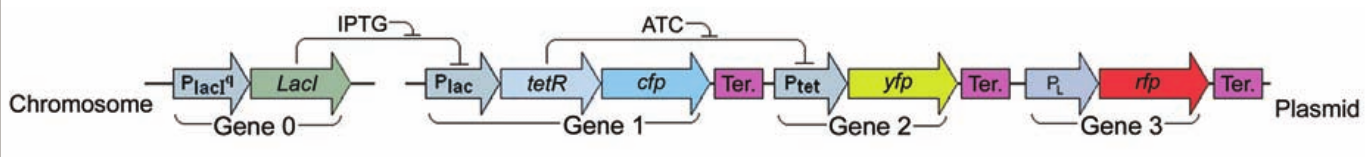
\includegraphics[width=15cm]{lan-circuit}
  \caption[Circuit used for the Langevin model]{\label{fig:lan-circuit} Circuit used in the Langevin model (from \cite{pedraza05}).}
\end{figure}

A similar effect happens on gene $2$, the tetracycline promoter P$_\text{tet}$, which regulated the expression of the yellow fluorescent protein \textit{yfp}. It is repressed by \textit{tetR} and the repressing effect of \textit{tetR} is also inhibited by ATC.

Therefore, both IPTG and ATC are environmental signals that are used to regulate the coupling between the different genes of the cascade. Notice that for instance, at higher quantities of IPTG, expression of gene $1$ is low since the repression over it is reduced. This also causes that without ATC, the expression of gene $2$ is high. 

The fluorescent proteins are used to quantify experimentally via fluorescence microscopy the expressions of each gene, which will be proportional to the intensity of the flourescence on each color. \textit{tetR} and \textit{cfp} are transcribed bicistronically in order to be able to quantify \textit{tetR} levels. We will assume that protein degradation is caused only by cell division (i.e. there is no active degradation). That allow us to use the same degradation constant for all proteins, and in particular, to assume that the behavior of \textit{cfp} reproduces exactly the behavior of \textit{tetR}. 

We will label the concentrations of \textit{LacI}, \textit{tetR} (and \textit{cfp}), \textit{yfp} and \textit{rfp} as $x_0$, $x_1$, $x_2$, and $x_3$, respectively.

\section{Mathematical derivations}

The differential equation for the mRNA will not be considered, we will write the equation for the proteins and include the effect of mRNA in the rate of creation $k$. The results of the previous chapter for the noise in proteins caused by mRNA will also be considered. The deterministic equation for the concentration of proteins of gene $0$ is 

\begin{equation}
\label{eq:detgene0}
\dot{x_0}(t) = k - \gamma x_0(t).
\end{equation}

Where now $k$ represents the average number of proteins created per unit time.\footnote{For a better understanding of this point. If we assume $\gamma_r\ll\gamma_p$, we can treat the mRNA in steady state, hence eq. \eqref{eq:mas-simple_det_2} becomes eq. \eqref{eq:detgene0} with $k \coloneqq k_p\langle n_1\rangle_s =  \frac{k_pk_r}{\gamma_r} = k_rb$.}In the Langevin approach noise terms are added to the previous equation representing the intrinsic noise $\mu_0(t)$ and the global noise $\xi_0(t)$. Hence, the equation for the stochastic process $x_0(t)$ is

\begin{equation}
\label{eq:gene0}
\dot{x_0}(t) = k - \gamma x_0(t) + \mu_0(t) + \xi_0(t).
\end{equation}

To find the correlations and the coefficient of variation, we need some information about the noise terms. First, the average of proteins $\langle x_0 \rangle (t)$ should follow the deterministic equation \eqref{eq:detgene0}, therefore

\begin{equation*}
\langle\mu_0\rangle(t) = \langle\xi_0\rangle(t) = 0.
\end{equation*}

Second, we will assume white noise statistics for both sources, that is, the values of the noise terms at different times are uncorrelated. Then

\begin{align}
\langle\mu_0(t)\mu_0(t+\tau)\rangle&=2\gamma(b_0+1)\bar{x}_0\delta(\tau),\label{eq:corin0}\\
\langle\xi_0(t)\xi_0(t+\tau)\rangle&=2\gamma\eta_G^2\bar{x}_0^2\delta(\tau). \label{eq:corex0}
\end{align}

\todo[inline]{Understand and explain more the constants and the assumption of white noise}

where $\eta_G$ is the strenght of the global noise, a parameter that is measured experimentally, and $b_0$ is the average number of protein produced per mRNA. In this section the bar denotes steady state average. Also, since both sources of noise are uncorrelated

\begin{equation}
\label{eq:corinex0}
\langle\mu_0(t)\xi_0(t+\tau)\rangle = 0.
\end{equation}

Define $\delta x_0 \coloneqq x_0 - \bar{x}_0$, replacing this on eq. \eqref{eq:gene0} we get

\begin{equation}
\frac{\mathrm{d}}{\mathrm{d}t}\left(\delta x_0(t) + \bar{x}_0\right) = k - \gamma (\delta x_0(t) + \bar{x}_0) + \mu_0(t) + \xi_0(t),
\end{equation}

Using the fact that $\bar{x}_0=k/\gamma$ we get

\begin{equation}
\label{eq:dgene0}
\dot{\delta x_0}(t) = -\gamma \delta x_0(t) + \mu_0(t) + \xi_0(t).
\end{equation}

We will Fourier transform the equation, find its square norm and use the Wiener-Khinchin theorem (eq. \eqref{eq:con-wkth}) to find the autocorrelations in terms of the power spectrum and to write the power spectrum of $\mu(t)$ and $\xi(t)$ in terms of their autocorrelations.

Taking the Fourier transform of eq. \eqref{eq:dgene0} and recalling that $[\mathscr{F}(\frac{\mathrm{d}x(t)}{\mathrm{d}t})](\omega) = i\omega \mathscr{F}(x(t))(\omega)$ for a function of time $x(t)$, we obtain after solving for $\hat{\delta x_0}$

\begin{equation}
\label{eq:fgene0}
\hat{\delta x_0}(\omega) = \frac{\hat{\mu_0}+\hat{\xi_0}}{\gamma + i\omega}.
\end{equation}

Taking the square norm and averaging we get

\begin{equation}
\left\langle |\hat{\delta x_0}|^2 \right\rangle = \frac{\left\langle|\hat{\mu_0}|^2\right\rangle + \left\langle\hat{\mu_0}^*\hat{\xi_0}\right\rangle+\left\langle\hat{\mu_0}\hat{\xi_0}^*\right\rangle+\left\langle|\hat{\xi_0}|^2\right\rangle}{\gamma^2 + \omega^2},
\end{equation}

And using the Wiener-Khinchin theorem and eqs. \eqref{eq:corin0} - \eqref{eq:corinex0}

\todo[inline]{Explain with more detail here}

\begin{equation}
  \label{eq:pgene0}
  \begin{split}
    \left\langle |\hat{\delta x_0}|^2 \right\rangle &= \frac{\left(2\gamma(b_0+1)\bar{x_0}+ 2\gamma\eta_G^2\bar{x_0}^2\right)\mathscr{F}(\delta(t))}{\gamma^2+\omega^2}\\
    &=\frac{2\gamma\bar{x_0}^2\left(\nicefrac{(b_0+1)}{\bar{x_0}}+ \eta_G^2\right)}{\gamma^2+\omega^2},
  \end{split}
\end{equation}

where the cross terms are zero by eq. \eqref{eq:corinex0}. Applying the inverse Fourier transform at $t=0$ we get

\begin{equation*}
\langle \delta x_0^2 \rangle = 2\gamma\bar{x_0}^2\left(\nicefrac{(b_0+1)}{\bar{x_0}}+ \eta_G^2\right)\frac{1}{2\pi}\int_{-\infty}^{\infty}\frac{d\omega}{\omega^2+\gamma^2}
\end{equation*}

The integral can be easily solved by residues resulting in $\pi/\gamma$, therefore

\begin{equation*}
\langle \delta x_0^2 \rangle = \bar{x_0}^2\left(\frac{(b_0+1)}{\bar{x_0}}+ \eta_G^2\right)
\end{equation*}

And dividing by $\bar{x_0}^2$, we obtain the coefficient of variation

\begin{equation}
  \label{eq:etagene0}
  \boxed{\eta_0^2 = \frac{(b_0+1)}{\bar{x_0}}+ \eta_G^2 = \eta_{0\text{int}}^2+\eta_G^2}.
\end{equation}

This approach enabled us to explicitly separate the total noise of gene $0$ in the intrinsic and the extrinsic part. Now we will make the calculation for gene $1$, which follows the equation.

\begin{equation}
\label{eq:gene1}
\dot{x_1}(t) = k_1(x_{0A})-\gamma x_1+\mu_1+\xi_1
\end{equation}

The decay rate $\gamma$ is the same for gene $1$ than for gene $0$ after making the assumption that the decay depends only on dilution due to cellular growth. The creation rate $k_1$ is a Hill equation for activation. The statistics for the noise terms are analogous to eqs. \eqref{eq:corin0} - \eqref{eq:corinex0}. We also need to know in this case the correlations between the noise terms corresponding to gene $0$ and the ones corresponding to gene $1$. As we have said, extrinsic sources of noise are uncorrelated

\todo[inline]{Explain more about the dilution, perhaps before}

\begin{equation}
\label{eq:corcross01}
\langle\mu_0(t)\mu_1(t+\tau)\rangle = \langle\mu_0(t)\xi_1(t+\tau)\rangle = \langle\mu_1(t)\xi_0(t+\tau)\rangle = 0,
\end{equation}

but the extrinsic parts of the noise of genes $0$ and $1$ are correlated. In analogy with eq. \eqref{eq:corex0} we get

\begin{equation}
  \langle\xi_0(t)\xi_1(t+\tau)\rangle = 2\gamma\eta_G^2\bar{x_0}\bar{x_1}\delta(\tau).
\end{equation}

\todo[inline]{Also, understand and explain the q term here}

We proceed in a similar way to gene $0$. Defining $\delta x_1(t) \coloneqq x_1(t) - \bar{x_1}$, writing eq. \eqref{eq:gene1} in terms of $\delta x_1$, $\delta x_{0A}$, and making a Taylor expansion of $f_1$ to first order in $x_{0A}$ about $\bar{x}_{0A}$ we obtain.

\begin{equation}
\dot{\delta x_1} = k_1(\bar{x_{0A}}) + \left.\frac{dk_1(x_{0A})}{dx_{0A}}\right|_{\bar{x_{0A}}}\delta x_{0A} - \gamma(\delta x_1 + \bar{x_1}) + \mu_1 + \xi_1,
\end{equation}

but from eq. \eqref{eq:gene1} we can see that $\bar{x_1} = \nicefrac{k_1(\bar{x_{0A}})}{\gamma}$, therefore

\begin{equation}
  \label{eq:dgene1}
  \dot{\delta{x_1}(t)}=c_1\delta x_{0A}-\gamma\delta x_1 + \mu_1 \xi_1,
\end{equation}

where $c_1 \coloneqq \left.\nicefrac{dk_1(x_{0A})}{dx_{0A}}\right|_{\bar{x_{0A}}}$ Fourier transforming and solving for $\hat{\delta x_1}$ we get

\begin{equation*}
  \hat{\delta x_1}=\frac{c_1\hat{\delta x_{0A}}+\hat{\mu_1}+\hat{\xi_1}}{\gamma + i\omega}.
\end{equation*}

Taking the square norm and averaging

\begin{equation*}
  \label{eq:pgene1}
  \begin{split}
    \left\langle|\hat{\delta x_1}|^2\right\rangle &= \frac{1}{\omega^2+\gamma^2}\left(c_1\hat{\delta x_{0A}} + \hat{\mu_1} + \hat{\xi_1}\right)\left(c_1\hat{\delta x_{0A}}^* + \hat{\mu_1}^* + \hat{\xi_1}^*\right)\\
    &=\frac{1}{\omega^2+\gamma^2}\left(c_1^2 \left\langle|\hat{\delta x_{0A}}|^2\right\rangle + c_1\left(\langle\hat{\delta x_{0A}}\hat{\xi_1}^*\rangle+\langle\hat{\delta x_{0A}}^*\hat{\xi_1}\rangle\right) +  \left\langle|\hat{\mu_1}|^2\right\rangle +  \left\langle|\hat{\xi_1}|^2\right\rangle\right)
  \end{split}
\end{equation*}

Using the Wiener-Khinchin theorem and the equations for the correlations we get

\begin{align*}
  \left\langle|\hat{\mu_1}|^2\right\rangle &= 2\gamma(b_1+1)\bar{x_1},\\
  \left\langle|\hat{\xi_1}|^2\right\rangle &= 2\gamma\eta_G^2\bar{x_1}^2,
\end{align*}

since the Fourier transform of the Dirac delta is $1$. Also, from eqs. \eqref{eq:fgene0} and \eqref{eq:pgene0} we get

\begin{align*}
\left\langle|\hat{\delta x_{0A}}|^2\right\rangle &= \frac{2\gamma\bar{x_0}^2\left(\nicefrac{(b_0+1)}{\bar{x_0}}+ \eta_G^2\right)}{\gamma^2+\omega^2},\\
\langle\hat{\delta x_{0A}}\hat{\xi_1}^*\rangle &= \frac{1}{\gamma+i\omega}\left(\langle\hat{\mu_0}\hat{\xi_1}^*\rangle + \langle\hat{\xi_0}\hat{\xi_1}^*\rangle \right) = \frac{\langle\hat{\xi_0}\hat{\xi_1}^*\rangle}{\gamma+i\omega}\\
\langle\hat{\delta x_{0A}}^*\hat{\xi_1}\rangle &= \frac{1}{\gamma-i\omega}\left(\langle\hat{\mu_0}^*\hat{\xi_1}\rangle + \langle\hat{\xi_0}^*\hat{\xi_1}^*\rangle \right) = \frac{\langle\hat{\xi_0}^*\hat{\xi_1}\rangle}{\gamma-i\omega}
\end{align*}

Where the last step in the last two equations comes from the Wiener-Khinchin theorem and eq. \eqref{eq:corcross01}. Replacing the previous equations in eq. \eqref{eq:pgene1} and taking the inverse transform we get for the variance

\begin{equation}
  \begin{split}
    \langle \delta x_1^2\rangle &= 2\gamma\bar{x_0}^2c_1^2\left(\nicefrac{(b_0+1)}{\bar{x_0}}+ \eta_G^2\right)\frac{1}{2\pi}\int_{-\infty}^{\infty}\frac{d\omega}{(\omega^2+\gamma^2)^2}\\
    &+2\gamma\eta_G^2\bar{x_0}\bar{x_1}c_1\frac{1}{2\pi}\left(\int_{-\infty}^{\infty}\frac{d\omega}{(\gamma + i\omega)(\omega^2+\gamma^2)} + \int_{-\infty}^{\infty}\frac{d\omega}{(\gamma - i\omega)(\omega^2+\gamma^2)}\right)\\
    &+2\gamma\bar{x_1}^2 \left(\nicefrac{(b_1+1)}{\bar{x_1}}+\eta_G^2\right)\frac{1}{2\pi}\int_{-\infty}^{\infty}\frac{d\omega}{\omega^2+\gamma^2}.
  \end{split}
\end{equation} 

Solving the integrals in the complex plane and rearranging

\begin{equation}
  \langle \delta x_1^2\rangle = \frac{c_1^2\bar{x_0}^2}{2\gamma^2}\left(\nicefrac{(b_0+1)}{\bar{x_0}}+ \eta_G^2\right) + \frac{c_1\eta_G^2\bar{x_0}\bar{x_1}}{\gamma} + \bar{x_1}^2\left(\nicefrac{(b_1+1)}{\bar{x_1}}+\eta_G^2\right).
\end{equation}

Writing in terms of the logarithmic gain $H_{ji}\coloneqq -\frac{\langle x_i\rangle}{\langle x_j\rangle}\frac{1}{\gamma_j}\frac{\mathrm{d} f_j(x_i)}{\mathrm{d}x_i}$, in this case it becomes $H_{10}=-\frac{c_1\bar{x_0}}{\gamma x_1}$. Dividing by $\bar{x_1}^2$ and rearranging

\begin{equation}
  \label{eq:etagene1}
  \boxed{\eta_1^2 = \eta_{1\text{int}}^2 + \frac{1}{2}H_{10}^2\eta_0^2+\eta_G^2\left(1-H_{10}\right)}.
\end{equation}

\todo[inline]{TODO: Explain a lot more about the logarithmic gain}

Where $\eta_{1\text{int}}^2 = \nicefrac{(b_1+1)}{\bar{x_1}}$ and $\eta_0^2$ is given by eq. \ref{eq:etagene0}.

The result can be interpreted as follows, the total noise in gene one is given by the intrinsic part, the noise from gene $0$ that is propagated to gene $1$ (including both its intrinsic and global part) and the global noise that enters directly into gene $1$. The factor of $1/2$ arises from the time averaging since we assumed equal degradation rates for both proteins.

\todo[inline]{See if it is better to do it with different gammas}

For gene $2$ we proceed similarly, with analogous statistics for the noise terms, the resulting noise is

\begin{equation}
  \label{eq:etagene2}
  \boxed{\eta_2^2 = \eta_{2\text{int}}^2 + \frac{1}{2}H_{21}^2\eta_1^2+\frac{1}{8}H_{21}^2H_{10}^2\eta_0^2+\eta_G^2\left(1-H_{21}-\frac{1}{4}H_{21}^2H_{10}+\frac{1}{2}H_{21}H_{10}\right)}.
\end{equation}

Which contains the intrinsic noise of gene $2$, the contribution from the total noise of gene $1$, the contribution from the total noise of gene $0$ that is transmitted first to gene $1$ and then to gene $2$ and the global noise that enters directly. 

The correlations can be found in a similar fashion.

\todo[inline]{TODO: Find the correlations and do the analysis that JM did on SysBio class}

\section{Explicit expressions for the logarithmic gain}



\section{Analysis and implications}

As it can be noticed in eqs. \eqref{eq:etagene0}, \eqref{eq:etagene1} and \eqref{eq:etagene2}, the noise propagation follows the sequence of fig. \ref{fig:lan-noise_sources}. For each gene there is an independent intrinsic noise a correlated global noise, and both the transmitted global and intrinsic noise between the genes of the cascade whose strenght is determined by the logarithmic gain $H$.

\begin{figure}[H]
  \centering
  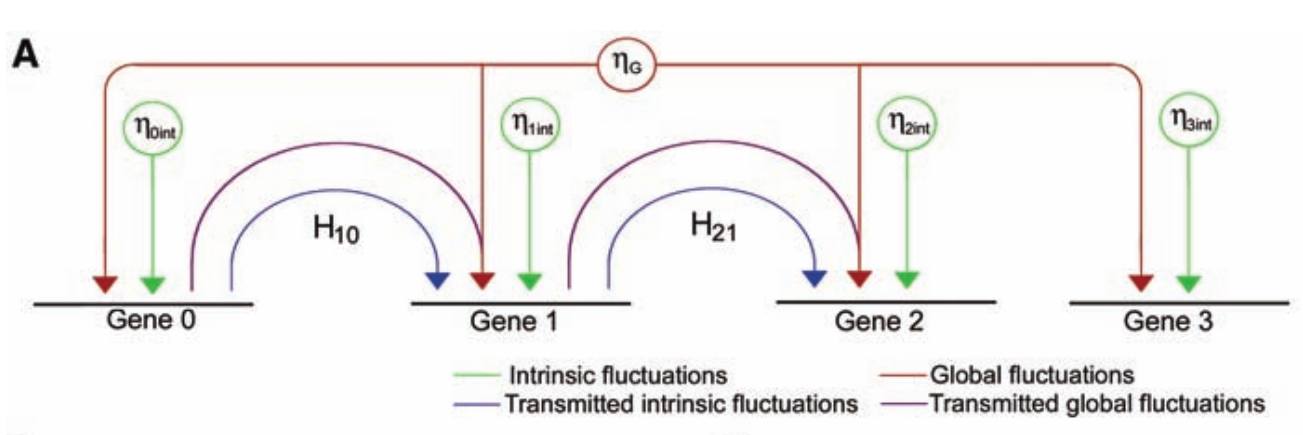
\includegraphics[width=15cm]{lan-noise_sources}
  \caption[Propagation of noise through a cascade]{\label{fig:lan-noise_sources} Different sources of noise and their propagation along the cascade of regulation (from \cite{pedraza05}).}
\end{figure}

\todo[inline]{TODO: Analyze the results physically (recall SysBio class), reproduce the graphics and analyze them}

This approach enables us to calculate the coefficient of variation for a cascade of regulation and separate the different sources of noise. Also, it enables to write the effect of the upstream genes in terms of the logarithmic gain, making it very intuitive. The results of the theoretical model were tested with experiments where the genes that are part of the cascade are transcribed bicistronicaly with fluorescent reporters. The fluctuations in the intensity of the reporters was used to measure the noise in the population of cells.
